
\section*{CHƯƠNG 2. PHÂN TÍCH HỆ THỐNG}
\setcounter{section}{2}
\setcounter{subsection}{0} %LƯU Ý MỖI LẦN THÊM CHƯƠNG MỚI CẦN THÊM CÂU NÀY ĐỂ RESET THỨ TỰ CỦA SUBSECTON VỀ 1
\setcounter{table}{0} % LƯU Ý SAU MỖI LẦN GỌI BẢNG HAY HÌNH ẢNH PHẢI THÊM CÂU NÀY ĐỂ RESET THỨ TỰ
\setcounter{figure}{0} %% LƯU Ý SAU MỖI LẦN GỌI BẢNG HAY HÌNH ẢNH PHẢI THÊM CÂU NÀY ĐỂ RESET THỨ TỰ
\addcontentsline{toc}{section}{\numberline{}CHƯƠNG 2. PHÂN TÍCH HỆ THỐNG}
Trong chương này, chúng em sẽ tiến hành phân tích hệ thống cho dự án đề tài "Hệ thống theo dõi và quản lý dữ liệu điện tim" dựa trên các mục tiêu
đã nêu ra trong Mục Đề xuất hệ thống ở Phần mở đầu. Trước tiên bài toán đặt ra ở hệ thống là:
\begin{adjustwidth}{1.5em}{}
\begin{itemize}
  \item Một ứng dụng để có thể giúp người dùng/bệnh nhân theo dõi được những thông tin cần về sức khoẻ tim mạch
  \item Trực quan và tiêu chuẩn hoá những thông tin đo được
    bằng hình ảnh hoặc số liệu để bác sĩ có thể dựa vào đó để đưa ra những đánh giá cho người dùng. Ngoài ra những thông tin này
    có thể hữu ích trong việc theo dõi sức khỏe tim mạch, theo dõi hiệu quả của liệu pháp 
    và hỗ trợ quyết định của người dùng
  \item Quản trị viên sẽ là người có thể phân công bác sĩ để chăm sóc, theo dõi sức khoẻ từ
  xa cho bệnh nhân
\end{itemize}
\end{adjustwidth}
Chi tiết về việc phân tích các yêu cầu hệ thống sẽ được chúng em trình bày ở các chương dưới.

\subsection{Sơ đồ use case}
\subsubsection{Use case tổng quát hệ thống}
Dựa vào những phân tích về yêu cầu chức năng, các use case trong hệ thống được chúng em thể hiện ở hình dưới 
  \begin{figure}[H]
    \centering
    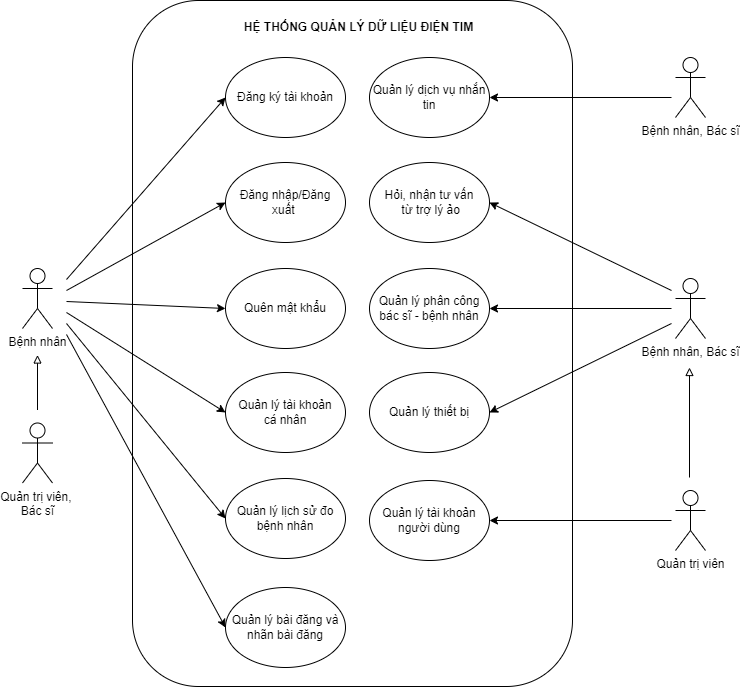
\includegraphics[width=16cm,height=14cm]{Images/use_case/use_case_general.png}
    \caption[Sơ đồ use case tổng quát của hệ thống]{\bfseries \fontsize{12pt}{0pt}
    \selectfont Sơ đồ use case tổng quát của hệ thống}
    \label{use_case_general} %đặt tên cho ảnh
  \end{figure}

\subsubsection{Use case chức năng xem lịch sử các lần đo}
  \begin{figure}[H]
    \centering
    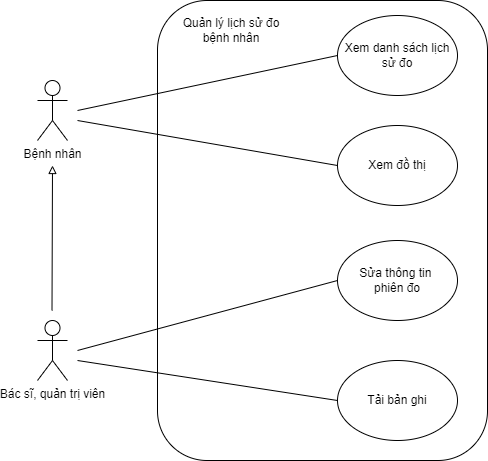
\includegraphics[width=12cm,height=4.8cm]{Images/use_case/use_case_view_history_record.png}
    \caption[Sơ đồ use case chức năng xem lịch sử các lần đo]{\bfseries \fontsize{12pt}{0pt}
    \selectfont Sơ đồ use case chức năng xem lịch sử các lần đo}
    \label{use_case_view_history_record} %đặt tên cho ảnh
  \end{figure}

  \begin{table}[H]
    \caption{\bfseries \fontsize{12pt}{0pt}\selectfont Bảng phân tích use case chức năng xem lịch sử các lần đo}
    \centering
    \begin{tabularx}{0.9\textwidth}{|c|X|}
      \hline
      \textbf{Tên chức năng} & \textbf{Xem lịch sử các lần đo} \\
      \hline
      Tác nhân & Bệnh nhân, Bác sĩ \\
      \hline
      Mô tả & Cho phép bệnh nhân xem lịch sử các lần đo điện tim và bác sĩ xem được lịch sử các lần đo của bệnh nhân
      mà mình quản lý \\
      \hline
      Điều kiện trước & Người dùng cần có kết nối Internet và đã đăng nhập \\
      \hline
      Dòng sự kiện chính & 
      % \begin{tabular}{@{}l@{}}
        Chi tiết luồng sự kiện được thể hiện ở Hình \ref{view_record_timeline}, Hình \ref{getEcgRecordsByUserId}, Hình \ref{getEcgRecordsByDoctor} 
        \\
      % \end{tabular} \\
      \hline
    \end{tabularx}
  \end{table}
% \newpage
\subsection{Thẻ CRC (Class - Responsibility - Collaboration Card)}

% \newpage
\subsection{Sơ đồ lớp}

% \newpage
\subsection{Sơ đồ tuần tự}
Để phân tích cụ thể hơn từng luồng trong hệ thống qua use case, chúng em xin phép được trình bày các sơ đồ tuần
tự. 
\subsubsection{Sơ đồ tuần tự chức năng đăng ký}
  \begin{figure}[H]
        \centering
        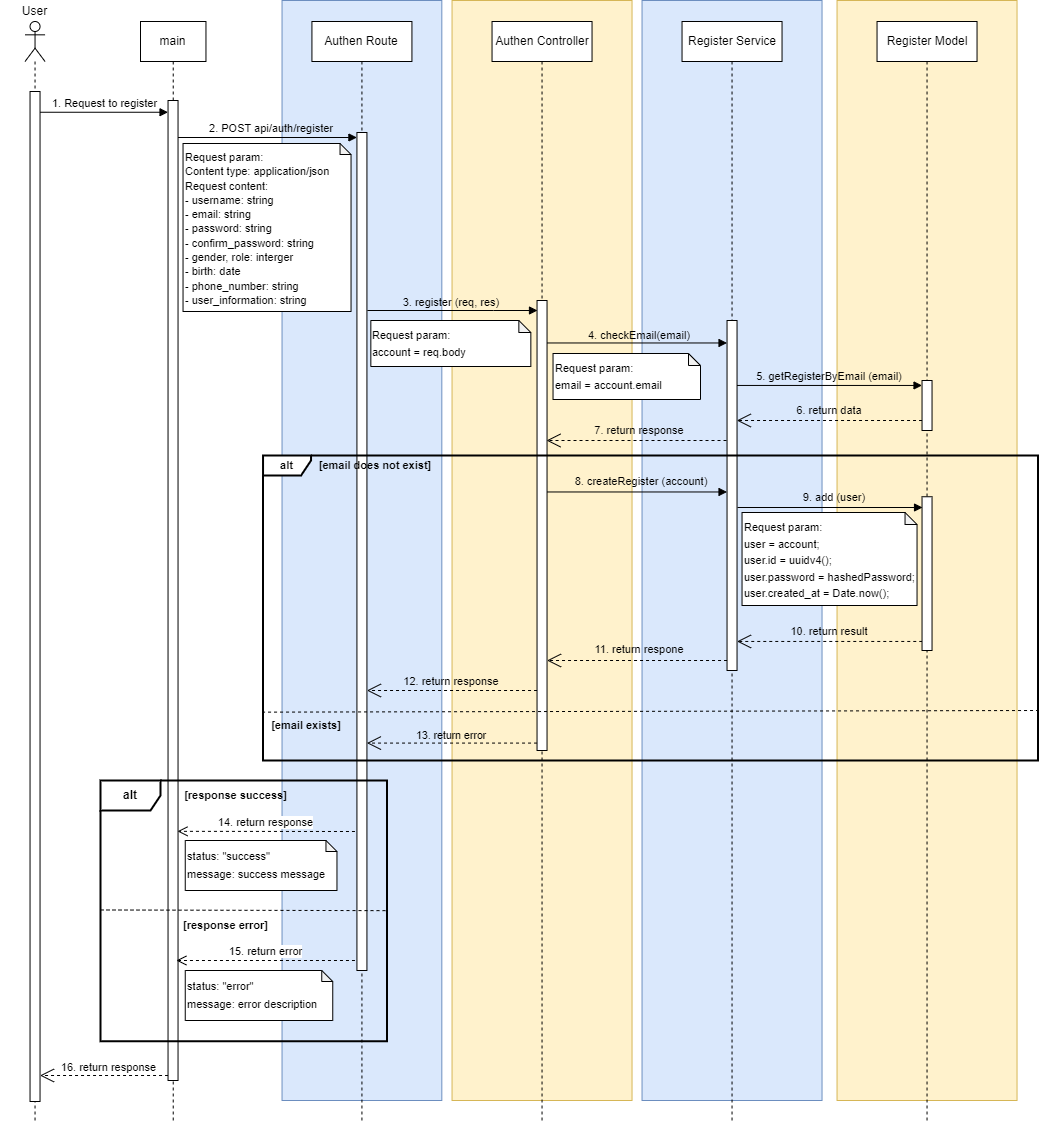
\includegraphics[width=12.9cm,height=9.4cm]{Images/mobile_app/register.png}
        \caption[Sơ đồ tuần tự chức năng đăng ký trên App]{\bfseries \fontsize{12pt}{0pt}
        \selectfont Sơ đồ tuần tự chức năng đăng ký trên App}
        \label{register} %đặt tên cho ảnh
  \end{figure}
  Sơ đồ tuần tự trên mô tả chi tiết quá trình người dùng đăng ký vào hệ thống. Người dùng gửi yêu cầu đăng ký, yêu cầu sẽ
  được xử lý bởi Control, nếu có lỗi phát sinh sẽ trả ra lỗi cho người dùng và yêu cầu người dùng nhập lại. Control
  sẽ xử lý cụ thể như thế nào được chúng em thể hiện trong Hình \ref{backend_register} trong chương sau.
\subsubsection{Sơ đồ tuần tự chức năng đăng nhập/đăng xuất}

    \begin{figure}[H]
         \centering
         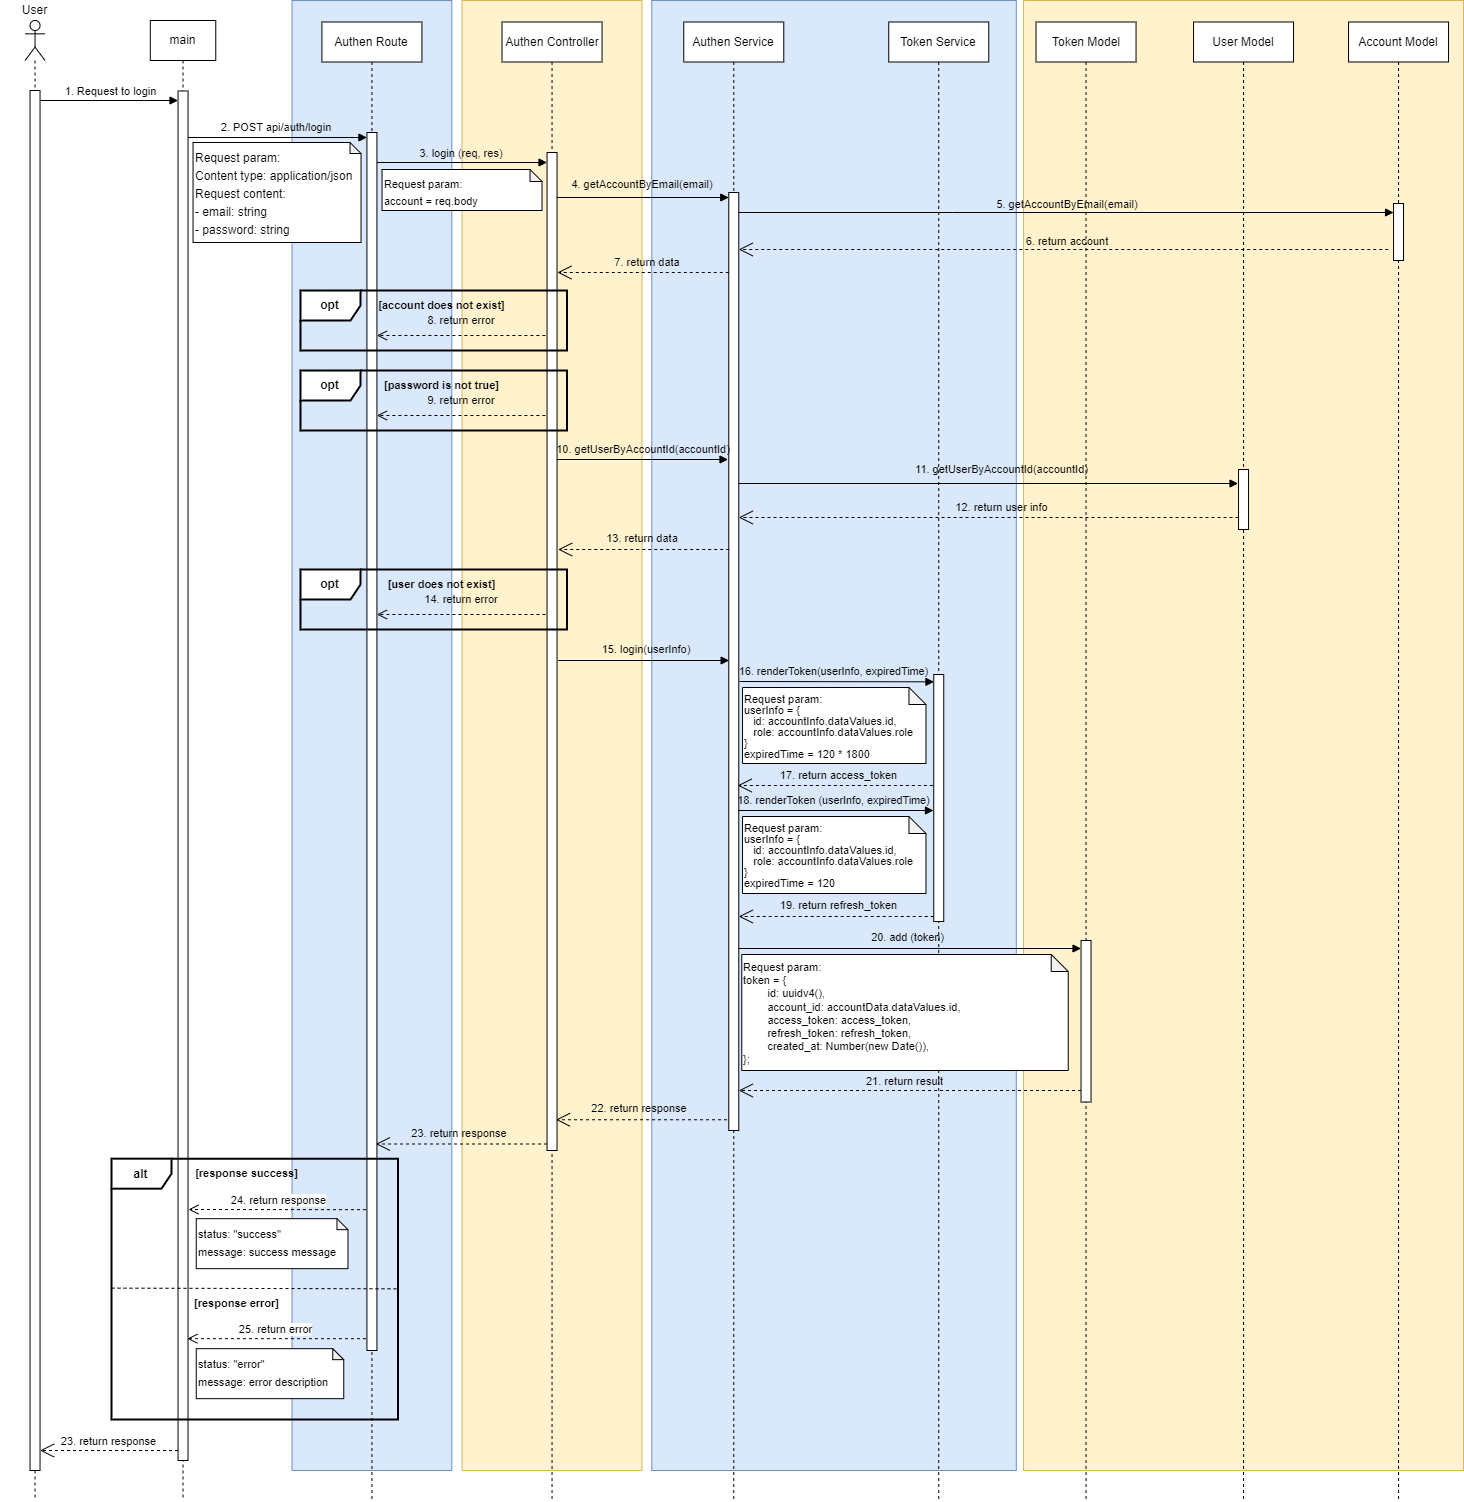
\includegraphics[width=16cm,height=12cm]{Images/mobile_app/login.png}
         \caption[Sơ đồ tuần tự chức năng đăng nhập trên App]{\bfseries \fontsize{12pt}{0pt}
         \selectfont Sơ đồ tuần tự chức năng đăng nhập trên App}
         \label{login} %đặt tên cho ảnh
    \end{figure}

  Sơ đồ tuần tự trên mô tả chi tiết quá trình người dùng đăng nhập vào hệ thống. Người dùng gửi yêu cầu đăng nhập, yêu cầu sẽ
  được xử lý bởi Control, nếu có lỗi phát sinh sẽ trả ra lỗi cho người dùng và yêu cầu người dùng nhập lại. Việc Control
  sẽ xử lý cụ thể yêu cầu người dùng được chúng em thể hiện trong Hình \ref{backend_login} trong chương sau.

  \begin{figure}[H]
    \centering
    \includegraphics[width=12cm,height=6cm]{Images/mobile_app/logout.png}
    \caption[Sơ đồ tuần tự chức năng đăng xuất trên App]{\bfseries \fontsize{12pt}{0pt}
    \selectfont Sơ đồ tuần tự chức năng đăng xuất trên App}
    \label{logout} %đặt tên cho ảnh
\end{figure}

Sơ đồ tuần tự trên mô tả chi tiết quá trình người dùng đăng xuất khỏi hệ thống. Người dùng gửi yêu cầu đăng xuất, yêu cầu sẽ
được xử lý bởi Control, nếu có lỗi phát sinh sẽ trả ra lỗi cho người dùng và yêu cầu người dùng nhập lại. Việc Control
sẽ xử lý cụ thể yêu cầu người dùng được chúng em thể hiện trong Hình \ref{backend_logout} trong chương sau.

\subsection{Phân tích dữ liệu}

Tại phần này, chúng em sẽ tiến hành xác định và mô tả các thực thể cũng như
 thuộc tính quan trọng trong hệ thống. Việc này giúp chúng ta có cái
  nhìn tổng quan về các yếu tố chính cần được quản lý và lưu trữ
   trong cơ sở dữ liệu. Bằng cách làm điều này, chúng ta có thể
    xây dựng một mô hình dữ liệu cơ bản để hỗ trợ việc thiết kế và
     triển khai hệ thống một cách hiệu quả.

     Trước hết, chúng em sẽ xác định và mô tả các thực thể chính trong hệ
      thống. Thực thể là các đối tượng hoặc khái niệm quan
       trọng mà chúng ta cần theo dõi và quản lý. Sau đó, chúng ta sẽ xác
        định các thuộc tính liên quan đến mỗi thực thể, các thông tin cần
         được lưu trữ và quản lý.

\begin{table}[H]
  \caption{\bfseries \fontsize{12pt}{0pt}\selectfont Bảng thực thể và thuộc tính}
  \centering
  \begin{tabularx}{0.9\textwidth}{|c|X|}
    \hline
    \textbf{Thực thể} & \textbf{Thuộc tính} \\
    \hline
    Người dùng & 
    ID người dùng, ID tài khoản, Tên người dùng, Email, Mật khẩu, Ngày sinh, Giới tính, Số điện thoại, Quyền, Thông tin người dùng \\
    \hline
    Token đăng nhập &
    ID token, ID tài khoản, Token truy cập, Token làm mới \\
    \hline
    Thiết bị & 
    ID thiết bị, ID người dùng thiết bị, ID bác sĩ theo dõi, Tên thiết bị, Loại thiết bị, Thông tin thiết bị, Trạng thái thiết bị, Ngày bắt đầu sử dụng\\
    \hline
    Các tần số đo được của thiết bị &
    ID tần số, ID thiết bị, Tên loại tần số, Thông tin, Giá trị đo được \\
    \hline
    Bản ghi ECG & 
    ID bản ghi ECG, ID người dùng, ID thiết bị, Loại bản ghi, Đường dẫn lưu trữ dữ liệu, Thời gian bắt đầu đo, Thời gian kết thúc đo \\
    \hline
    Thông tin đoạn hội thoại &
    ID đoạn hội thoại, Tên đoạn hội thoại, Loại đoạn hội thoại, Đường dẫn avatar đoạn hội thoại \\
    \hline
    Thành viên tham gia hội thoại &
    ID đoạn hội thoại, ID người dùng tham gia, Trạng thái thông báo (Có thông báo, Không thông báo), Tác vụ (người tạo đoạn hội thoại, thành viên trong đoạn hội thoại), Trạng thái đã xem\\
    \hline
    Tin nhắn & 
    ID tin nhắn, ID đoạn hội thoại, ID người gửi, Các tệp đính kèm, Tin nhắn hệ thống, Ghim (tin nhắn được ghim, không được ghim), Thời gian ghim tin nhắn, Các lượt thả cảm xúc \\
    \hline
    Tệp đính kèm &
    ID tệp đính kèm, ID tin nhắn, ID đoạn hội thoại, Đường dẫn nội dung, Tên tệp, Kích thước tệp, Đường dẫn thumbnail, Loại đính kèm (hình ảnh, video, tệp tin) \\
    \hline
    Hội thoại với AI &
    ID hội thoại, ID người gửi, Nội dung chat, Dữ liệu đầu vào \\
    \hline 
    Phân công bệnh nhân - bác sĩ & 
    ID phân công, ID bệnh nhân, ID bác sĩ, Ngày bắt đầu, Ngày kết thúc \\
    \hline
    Danh mục tin tức &
    ID danh mục tin tức, Tên danh mục tin tức, Mô tả danh mục tin tức \\
    \hline
    Tin tức &
    ID tin tức, Tiêu đề, Nội dung, ID danh mục tin tức, Tác giả, Đường dẫn, Đường dẫn hình ảnh \\
    \hline
  \end{tabularx}

  
\end{table}
Sau khi hoàn thành được bảng thực thể và thuộc tính, chúng em xác định được mô hình thực thể liên kết như sau:

\begin{figure}[H]
  \centering
  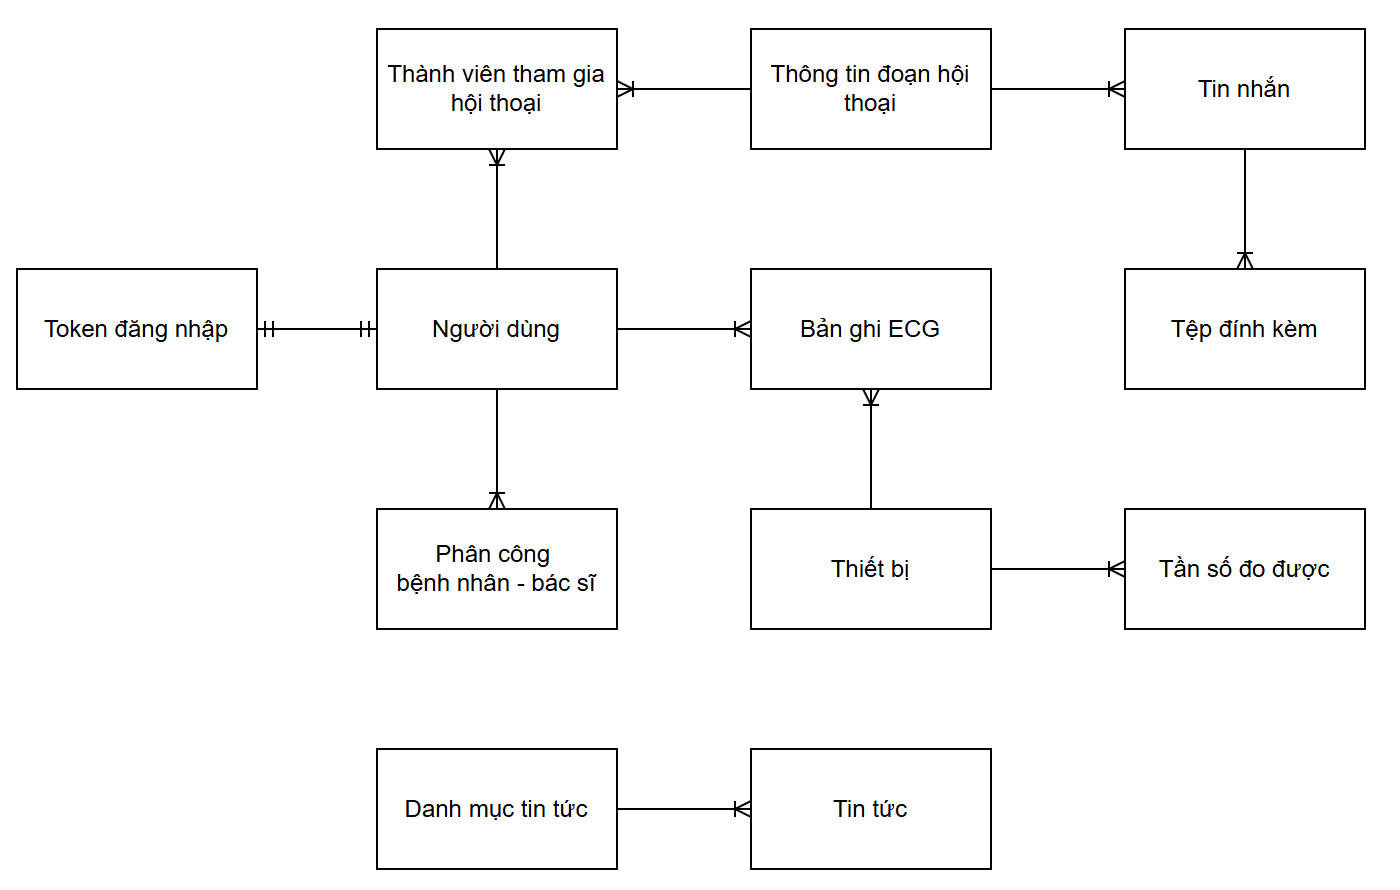
\includegraphics[width=15cm,height=8cm]{Images/system/fmECG_connection_entity.png}
  \caption[Mô hình thực thể liên kết]{\bfseries \fontsize{12pt}{0pt}
  \selectfont Mô hình thực thể liên kết}
  \label{ttlk} %đặt tên cho ảnh
\end{figure}

\subsection{Thiết kế cơ sở dữ liệu}
\subsubsection{Chuyển mô hình thực thể liên kết sang mô hình quan hệ}

\begin{itemize}
  \item Người dùng (\textbf{ID người dùng}, ID tài khoản, Tên người dùng, Email, Mật khẩu, Ngày sinh, Giới tính, Số điện thoại, Quyền, Thông tin người dùng)
  \item Token đăng nhập (\textbf{ID token}, ID tài khoản, Token truy cập, Token làm mới)
  \item Thiết bị (\textbf{ID thiết bị}, ID người dùng thiết bị, ID bác sĩ theo dõi, Tên thiết bị, Loại thiết bị, Thông tin thiết bị, Trạng thái thiết bị, Ngày bắt đầu sử dụng)
  \item Bản ghi ECG (\textbf{ID bản ghi ECG}, ID người dùng, ID thiết bị, Loại bản ghi, Đường dẫn lưu trữ dữ liệu, Thời gian bắt đầu đo, Thời gian kết thúc đo)
  \item Thông tin đoạn hội thoại (\textbf{ID đoạn hội thoại}, Tên đoạn hội thoại, Loại đoạn hội thoại, Đường dẫn avatar đoạn hội thoại)
  \item Thành viên tham gia hội thoại (\textbf{ID}, ID đoạn hội thoại, ID người dùng tham gia, Trạng thái thông báo, Tác vụ, Trạng thái đã xem)
  \item Tin nhắn (\textbf{ID tin nhắn}, ID đoạn hội thoại, ID người gửi, Các tệp đính kèm, Tin nhắn hệ thống, Ghim, Thời gian ghim tin nhắn, Các lượt thả cảm xúc)
  \item Tệp đính kèm (\textbf{ID tệp đính kèm}, ID tin nhắn, ID đoạn hội thoại, Đường dẫn nội dung, Tên tệp, Kích thước tệp, Đường dẫn thumbnail, Loại đính kèm)
  \item Hội thoại với AI (\textbf{ID hội thoại}, ID người gửi, Nội dung chat, Dữ liệu đầu vào)
  \item Phân công bệnh nhân - bác sĩ (\textbf{ID phân công}, ID bệnh nhân, ID bác sĩ, Ngày bắt đầu)
  \item Danh mục tin tức (\textbf{ID danh mục tin tức}, Tên danh mục tin tức, Mô tả danh mục tin tức)
  \item Tin tức (\textbf{ID tin tức}, Tiêu đề, Nội dung, ID danh mục tin tức, Tác giả, Đường dẫn, Đường dẫn hình ảnh)
\end{itemize}


\subsubsection{Chuẩn hoá 3NF}
Các bảng đã được thiết kế theo nguyên tắc chuẩn hoá 3NF, vì không có thuộc tính lặp lại và các thuộc tính không phụ thuộc vào một tập hợp con của khóa chính.

\paragraph{Chuẩn hoá bảng Người dùng}
\mbox{}

\begin{table}[H]
  \caption{\bfseries \fontsize{12pt}{0pt}\selectfont Bảng chuẩn hoá bảng Người dùng}
  \centering
  \begin{tabularx}{0.9\textwidth}{|X|X|}
    \hline
    \textbf{Danh sách thuộc tính} & ID người dùng, ID tài khoản, Tên người dùng, Email, Mật khẩu, Ngày sinh, Giới tính, Số điện thoại, Quyền, Thông tin người dùng \\
    \hline
    \textbf{Quy tắc nghiệp vụ} & \textbf{Phụ thuộc hàm} \\
    \hline
    Mỗi người dùng có một ID riêng, có duy nhất mật khẩu, email, tên, ngày sinh, số điện thoại, quyền,
    giới tính, thông tin & \parbox[t]{\linewidth}{$\text{ID người dùng} \rightarrow$ mật khẩu, email, tên, ngày sinh, số điện thoại, quyền, thông tin} \\
    \hline
    \multicolumn{2}{|X|}{$\Rightarrow \text{Khoá chính của bảng: ID người dùng}$} \\
    \multicolumn{2}{|X|}{$\Rightarrow \text{Bảng Người dùng đã ở 3NF}$} \\
    \hline
  \end{tabularx}
\end{table}

\paragraph{Chuẩn hoá bảng Token đăng nhập}
\mbox{}

\begin{table}[H]
  \caption{\bfseries \fontsize{12pt}{0pt}\selectfont Bảng chuẩn hoá bảng Token đăng nhập}
  \centering
  \begin{tabularx}{0.9\textwidth}{|X|X|}
    \hline
    \textbf{Danh sách thuộc tính} & ID token, ID tài khoản, Token truy cập, Token làm mới \\
    \hline
    \textbf{Quy tắc nghiệp vụ} & \textbf{Phụ thuộc hàm} \\
    \hline
    Mỗi người dùng có một ID token riêng, có duy nhất ID tài khoản, token truy cập và token làm mới 
    & \parbox[t]{\linewidth}{$\text{ID token} \rightarrow$ ID tài khoản, Token truy cập, Token làm mới} \\
    \hline
    \multicolumn{2}{|X|}{$\Rightarrow \text{Khoá chính của bảng: ID token đăng nhập}$} \\
    \multicolumn{2}{|X|}{$\Rightarrow \text{Bảng Token  đã ở 3NF}$} \\
    \hline
  \end{tabularx}
\end{table}

\paragraph{Chuẩn hoá bảng Thiết bị}
\mbox{}

\begin{table}[H]
  \caption{\bfseries \fontsize{12pt}{0pt}\selectfont Bảng chuẩn hoá bảng Thiết bị}
  \centering
  \begin{tabularx}{0.9\textwidth}{|X|X|}
    \hline
    \textbf{Danh sách thuộc tính} & ID thiết bị, ID người dùng thiết bị, ID bác sĩ theo dõi, Tên thiết bị, 
    Loại thiết bị, Thông tin thiết bị, Trạng thái thiết bị, Ngày bắt đầu sử dụng \\
    \hline
    \textbf{Quy tắc nghiệp vụ} & \textbf{Phụ thuộc hàm} \\
    \hline
    Mỗi thiết bị khi được sử dụng sẽ có một ID thiết bị riêng, có duy nhất tên thiết bị, loại thiết bị, thông tin thiết bị.
    ID người dùng thiết bị, ID bác sĩ theo dõi, trạng thái thiết bị, ngày bắt đầu sử dụng
    & \parbox[t]{\linewidth}{$\text{ID thiết bị} \rightarrow$ ID người dùng thiết bị, ID bác sĩ theo dõi, Tên thiết bị, 
    Loại thiết bị, Thông tin thiết bị, Trạng thái thiết bị, Ngày bắt đầu sử dụng} \\
    \hline
    \multicolumn{2}{|X|}{$\Rightarrow \text{Khoá chính của bảng: ID thiết bị}$} \\
    \multicolumn{2}{|X|}{$\Rightarrow \text{Bảng Thiết bị đã ở 3NF}$} \\
    \hline
  \end{tabularx}
\end{table}

\paragraph{Chuẩn hoá bảng Bản ghi ECG}
\mbox{}

\begin{table}[H]
  \caption{\bfseries \fontsize{12pt}{0pt}\selectfont Bảng chuẩn hoá bảng Bản ghi ECG}
  \centering
  \begin{tabularx}{0.9\textwidth}{|X|X|}
    \hline
    \textbf{Danh sách thuộc tính} & ID bản ghi ECG, ID người dùng, ID thiết bị, Loại bản ghi, 
    Đường dẫn lưu trữ dữ liệu, Thời gian bắt đầu đo, Thời gian kết thúc đo \\
    \hline
    \textbf{Quy tắc nghiệp vụ} & \textbf{Phụ thuộc hàm} \\
    \hline
    Mỗi bản ghi có một ID bản ghi ECG riêng, có duy nhất ID người dùng, ID thiết bị, Loại bản ghi, 
    Đường dẫn lưu trữ dữ liệu, Thời gian bắt đầu đo, Thời gian kết thúc đo
    & \parbox[t]{\linewidth}{$\text{ID bản ghi ECG} \rightarrow$ ID người dùng, ID thiết bị, Loại bản ghi, 
    Đường dẫn lưu trữ dữ liệu, Thời gian bắt đầu đo, Thời gian kết thúc đo} \\
    \hline
    \multicolumn{2}{|X|}{$\Rightarrow \text{Khoá chính của bảng: ID bản ghi ECG}$} \\
    \multicolumn{2}{|X|}{$\Rightarrow \text{Bảng Bản ghi ECG đã ở 3NF}$} \\
    \hline
  \end{tabularx}
\end{table}

\paragraph{Chuẩn hoá bảng Thông tin đoạn hội thoại}
\mbox{}

\begin{table}[H]
  \caption{\bfseries \fontsize{12pt}{0pt}\selectfont Bảng chuẩn hoá bảng Thông tin đoạn hội thoại}
  \centering
  \begin{tabularx}{0.9\textwidth}{|X|X|}
    \hline
    \textbf{Danh sách thuộc tính} & ID đoạn hội thoại, Tên đoạn hội thoại, 
    Loại đoạn hội thoại, Đường dẫn avatar đoạn hội thoại \\
    \hline
    \textbf{Quy tắc nghiệp vụ} & \textbf{Phụ thuộc hàm} \\
    \hline
    Mỗi đoạn hội thoại có một ID đoạn hội thoại riêng, có duy nhất tên đoạn hội thoại, 
    loại đoạn hội thoại, đường dẫn avatar đoạn hội thoại
    & \parbox[t]{\linewidth}{$\text{ID đoạn hội thoại} \rightarrow$ Tên đoạn hội thoại, 
    Loại đoạn hội thoại, Đường dẫn avatar đoạn hội thoại} \\
    \hline
    \multicolumn{2}{|X|}{$\Rightarrow \text{Khoá chính của bảng: ID đoạn hội thoại}$} \\
    \multicolumn{2}{|X|}{$\Rightarrow \text{Bảng Thông tin đoạn hội thoại đã ở 3NF}$} \\
    \hline
  \end{tabularx}
\end{table}

\paragraph{Chuẩn hoá bảng Thành viên tham gia hội thoại}
\mbox{}

\begin{table}[H]
  \caption{\bfseries \fontsize{12pt}{0pt}\selectfont Bảng chuẩn hoá bảng Thành viên tham gia hội thoại}
  \centering
  \begin{tabularx}{0.9\textwidth}{|X|X|}
    \hline
    \textbf{Danh sách thuộc tính} & ID, ID đoạn hội thoại, ID người dùng tham gia,
    Trạng thái thông báo, Tác vụ, Trạng thái đã xem \\
    \hline
    \textbf{Quy tắc nghiệp vụ} & \textbf{Phụ thuộc hàm} \\
    \hline
    Mỗi đoạn hội thoại có nhiều ID người dùng tham gia, mỗi người dùng có duy nhất trạng thái thông báo,
    tác vụ, trạng thái đã xem trong một đoạn hội thoại
    & \parbox[t]{\linewidth}{$\text{ID} \rightarrow$ ID đoạn hội thoại, ID người dùng tham gia,
    Trạng thái thông báo, Tác vụ, Trạng thái đã xem} \\
    \hline
    \multicolumn{2}{|X|}{$\Rightarrow \text{Khoá chính của bảng: ID}$} \\
    \multicolumn{2}{|X|}{$\Rightarrow \text{Bảng Thành viên tham gia hội thoại đã ở 3NF}$} \\
    \hline
  \end{tabularx}
\end{table}

\paragraph{Chuẩn hoá bảng Tin nhắn}
\mbox{}

\begin{table}[H]
  \caption{\bfseries \fontsize{12pt}{0pt}\selectfont Bảng chuẩn hoá bảng Tin nhắn}
  \centering
  \begin{tabularx}{0.9\textwidth}{|X|X|}
    \hline
    \textbf{Danh sách thuộc tính} & ID tin nhắn, ID đoạn hội thoại, ID người gửi, Các tệp đính kèm, 
    Tin nhắn hệ thống, Ghim, Thời gian ghim tin nhắn, Các lượt thả cảm xúc \\
    \hline
    \textbf{Quy tắc nghiệp vụ} & \textbf{Phụ thuộc hàm} \\
    \hline
    Mỗi tin nhắn có một ID tin nhắn riêng, thuộc một đoạn hội thoại, có duy nhất ID người gửi, các tệp đính kèm,
    tin nhắn hệ thống, ghim, thời gian ghim tin nhắn, các lượt thả cảm xúc
    & \parbox[t]{\linewidth}{$\text{ID tin nhắn} \rightarrow$ ID đoạn hội thoại, ID người gửi, các tệp đính kèm,
    tin nhắn hệ thống, ghim, thời gian ghim tin nhắn, các lượt thả cảm xúc} \\
    \hline
    \multicolumn{2}{|X|}{$\Rightarrow \text{Khoá chính của bảng: ID tin nhắn}$} \\
    \multicolumn{2}{|X|}{$\Rightarrow \text{Bảng Tin nhắn đã ở 3NF}$} \\
    \hline
  \end{tabularx}
\end{table}

\paragraph{Chuẩn hoá bảng Tệp đính kèm}
\mbox{}

\begin{table}[H]
  \caption{\bfseries \fontsize{12pt}{0pt}\selectfont Bảng chuẩn hoá bảng Tệp đính kèm}
  \centering
  \begin{tabularx}{0.9\textwidth}{|X|X|}
    \hline
    \textbf{Danh sách thuộc tính} & ID tệp đính kèm, ID tin nhắn, ID đoạn hội thoại, Đường dẫn nội
    dung, Tên tệp, Kích thước tệp, Đường dẫn thumbnail, Loại đính kèm \\
    \hline
    \textbf{Quy tắc nghiệp vụ} & \textbf{Phụ thuộc hàm} \\
    \hline
    Mỗi tệp đính kèm có một ID tệp đính kèm riêng, thuộc một tin nhắn trong một đoạn hội thoại, có duy nhất đường dẫn nội
    dung, tên tệp, kích thước tệp, đường dẫn thumbnail, loại đính kèm
    & \parbox[t]{\linewidth}{$\text{ID tệp đính kèm} \rightarrow$ ID tin nhắn, ID đoạn hội thoại, Đường dẫn nội
    dung, Tên tệp, Kích thước tệp, Đường dẫn thumbnail, Loại đính kèm} \\
    \hline
    \multicolumn{2}{|X|}{$\Rightarrow \text{Khoá chính của bảng: ID tệp đính kèm}$} \\
    \multicolumn{2}{|X|}{$\Rightarrow \text{Bảng Tệp đính kèm đã ở 3NF}$} \\
    \hline
  \end{tabularx}
\end{table}

\paragraph{Chuẩn hoá bảng Phân công bệnh nhân - bác sĩ}
\mbox{}

\begin{table}[H]
  \caption{\bfseries \fontsize{12pt}{0pt}\selectfont Bảng chuẩn hoá bảng Phân công bệnh nhân - bác sĩ}
  \centering
  \begin{tabularx}{0.9\textwidth}{|X|X|}
    \hline
    \textbf{Danh sách thuộc tính} & ID phân công, ID bệnh nhân, ID bác sĩ, Ngày bắt đầu \\
    \hline
    \textbf{Quy tắc nghiệp vụ} & \textbf{Phụ thuộc hàm} \\
    \hline
    Mỗi phân công bệnh nhân - bác sĩ có một ID phân công riêng, có duy nhất ID bệnh nhân, ID bác sĩ, ngày bắt đầu.
    Mỗi bệnh nhân thuộc một phân công duy nhất, còn mỗi bác sĩ có thể được giao nhiều phân công.
    & \parbox[t]{\linewidth}{$\text{ID phân công} \rightarrow$ ID bệnh nhân, ID bác sĩ, Ngày bắt đầu} \\
    \hline
    \multicolumn{2}{|X|}{$\Rightarrow \text{Khoá chính của bảng: ID phân công}$} \\
    \multicolumn{2}{|X|}{$\Rightarrow \text{Bảng Phân công bệnh nhân - bác sĩ đã ở 3NF}$} \\
    \hline
  \end{tabularx}
\end{table}

\paragraph{Chuẩn hoá bảng Danh mục tin tức}
\mbox{}

\begin{table}[H]
  \caption{\bfseries \fontsize{12pt}{0pt}\selectfont Bảng chuẩn hoá bảng Danh mục tin tức}
  \centering
  \begin{tabularx}{0.9\textwidth}{|X|X|}
    \hline
    \textbf{Danh sách thuộc tính} & ID danh mục tin tức, Tên danh mục tin tức, Mô tả danh mục tin tức \\
    \hline
    \textbf{Quy tắc nghiệp vụ} & \textbf{Phụ thuộc hàm} \\
    \hline
    Mỗi danh mục tin tức có một ID danh mục tin tức riêng, có duy nhất tên danh mục tin tức, mô tả danh mục tin tức
    & \parbox[t]{\linewidth}{$\text{ID danh mục tin tức} \rightarrow$ Tên danh mục tin tức, Mô tả danh mục tin tức} \\
    \hline
    \multicolumn{2}{|X|}{$\Rightarrow \text{Khoá chính của bảng: ID danh mục tin tức}$} \\
    \multicolumn{2}{|X|}{$\Rightarrow \text{Bảng Danh mục tin tức đã ở 3NF}$} \\
    \hline
  \end{tabularx}
\end{table}

\paragraph{Chuẩn hoá bảng Tin tức}
\mbox{}

\begin{table}[H]
  \caption{\bfseries \fontsize{12pt}{0pt}\selectfont Bảng chuẩn hoá bảng Tin tức}
  \centering
  \begin{tabularx}{0.9\textwidth}{|X|X|}
    \hline
    \textbf{Danh sách thuộc tính} & ID tin tức, Tiêu đề, Nội dung, ID danh mục tin tức, Tác giả, Đường dẫn,
    Đường dẫn hình ảnh \\
    \hline
    \textbf{Quy tắc nghiệp vụ} & \textbf{Phụ thuộc hàm} \\
    \hline
    Mỗi tin tức có một ID tin tức riêng, thuộc duy nhất một danh mục tin tức, có duy nhất tiêu đề, 
    nội dung, tác giả, đường dẫn, đường dẫn hình ảnh
    & \parbox[t]{\linewidth}{$\text{ID tin tức} \rightarrow$ Tiêu đề, Nội dung, ID danh mục tin tức, Tác giả, 
    Đường dẫn, Đường dẫn hình ảnh} \\
    \hline
    \multicolumn{2}{|X|}{$\Rightarrow \text{Khoá chính của bảng: ID tin tức}$} \\
    \multicolumn{2}{|X|}{$\Rightarrow \text{Bảng Tin tức đã ở 3NF}$} \\
    \hline
  \end{tabularx}
\end{table}

\subsection{Kết luận chương}

Trong chương này, chúng em đã thực hiện phân tích toàn diện về
 hệ thống cho đề tài , nhằm đáp ứng
  các mục tiêu và yêu cầu đã được đề xuất.

Chúng em đã xác định rõ ràng các khía cạnh quan trọng của hệ thống,
 tập trung vào việc thiết kế một hệ thống quản lý ECG hiệu quả,
  trực quan và có khả năng theo dõi sức khỏe tim mạch một cách
   chính xác. 


\newpage
